\documentclass[paper=a4, fontsize=11pt, UTF8]{article} % A4 paper and 11pt font size
\usepackage[a4paper,left=3.18cm,right=3.18cm,top=2.5cm,bottom=2.5cm]{geometry}
\usepackage{ctex}
%\usepackage[T1]{fontenc} % Use 8-bit encoding that has 256 glyphs
%\usepackage{fourier} % Use the Adobe Utopia font for the document - comment this line to return to the LaTeX default
\usepackage[english]{babel} % English language/hyphenation
\usepackage{amsmath,amsfonts,amsthm} % Math packages
\usepackage{graphicx}
%\usepackage{rotating} % for sidewaysfigure
\usepackage{listings}
\usepackage{xcolor}
\usepackage{siunitx}
\usepackage{booktabs}
\usepackage{multirow}
\usepackage{longtable}
\usepackage{hyperref}
\hypersetup{
    colorlinks,
    citecolor=black,
    filecolor=black,
    linkcolor=black,
    urlcolor=black
}

% Uncomment below to New page befor section
%\usepackage{titlesec}
%\newcommand{\sectionbreak}{\clearpage}
%\titleformat*{\section}{\centering \Large \bfseries}

\newcommand{\matr}[1]{\mathbf{#1}} % undergraduate algebra version
%\usepackage{sectsty} % Allows customizing section commands
%\allsectionsfont{\centering \normalfont\scshape} % Make all sections centered, the default font and small caps

\usepackage{fancyhdr} % Custom headers and footers
\pagestyle{fancyplain} % Makes all pages in the document conform to the custom headers and footers
\fancyhead[L]{}
\fancyhead[C]{}
\fancyhead[R]{\thepage} % No page header - if you want one, create it in the same way as the footers below
\fancyfoot[L]{} % Empty left footer
\fancyfoot[C]{\thepage} % Empty center footer
\fancyfoot[R]{} % Page numbering for right footer
%\renewcommand{\headrulewidth}{0pt} % Remove header underlines
\renewcommand{\footrulewidth}{0pt} % Remove footer underlines
\setlength{\headheight}{13.6pt} % Customize the height of the header

\numberwithin{equation}{section} % Number equations within sections (i.e. 1.1, 1.2, 2.1, 2.2 instead of 1, 2, 3, 4)
\numberwithin{figure}{section} % Number figures within sections (i.e. 1.1, 1.2, 2.1, 2.2 instead of 1, 2, 3, 4)
\numberwithin{table}{section} % Number tables within sections (i.e. 1.1, 1.2, 2.1, 2.2 instead of 1, 2, 3, 4)

%\setlength\parindent{0pt} % Removes all indentation from paragraphs - comment this line for an assignment with lots of text

\lstset{language=C++,%
    %basicstyle=\color{red},
    keywordstyle=\color{blue},%
    extendedchars=false,
    tabsize=4,
    breaklines,
    morekeywords=[2]{1}, keywordstyle=[2]{\color{black}},
    identifierstyle=\color{black},%
    stringstyle=\color{mylilas},
    commentstyle=\color{green},%
    frame=single,
    showstringspaces=false,%without this there will be a symbol in the places where there is a space
    numbers=left,%
    numberstyle={\small \color{black}},% size of the numbers
    numbersep=9pt, % this defines how far the numbers are from the text
    emph=[1]{for,end,break},emphstyle=[1]\color{red}, %some words to emphasise
    escapeinside=``
}


%\usepackage[framed,numbered,autolinebreaks,useliterate]{mcode}

\newcommand{\horrule}[1]{\rule{\linewidth}{#1}} % Create horizontal rule command with 1 argument of height

\title{
\normalfont \normalsize
\textsc{\kaishu 网络专题训练} \\ [5pt] % Your university, school and/or department name(s)
\horrule{0.5pt} \\[0.4cm] % Thin top horizontal rule
\huge 4over6隧道协议实验报告 \\ % The assignment title
\horrule{2pt} \\[0.5cm] % Thick bottom horizontal rule
}

\author{马 \;  也\quad 2013011365 \quad 计34\\ 沈哲言\quad 2013011371 \quad 计34}
%\author{马也} % Your name
\date{\normalsize\today} % Today's date or a custom date

\begin{document}

\maketitle % Print the title

% \thispagestyle{empty}
% \newpage

%\setcounter{page}{1}
%\tableofcontents
\fontsize{11pt}{18pt}\selectfont
%\newpage

\section{实验目的}

\begin{itemize}
\item 掌握Android下应用程序开发环境的搭建和使用
\item 掌握IPv4 over IPv6隧道的工作原理
\end{itemize}


\section{实验原理}

\subsection{4over6隧道模式原理}

\begin{figure}[htp]
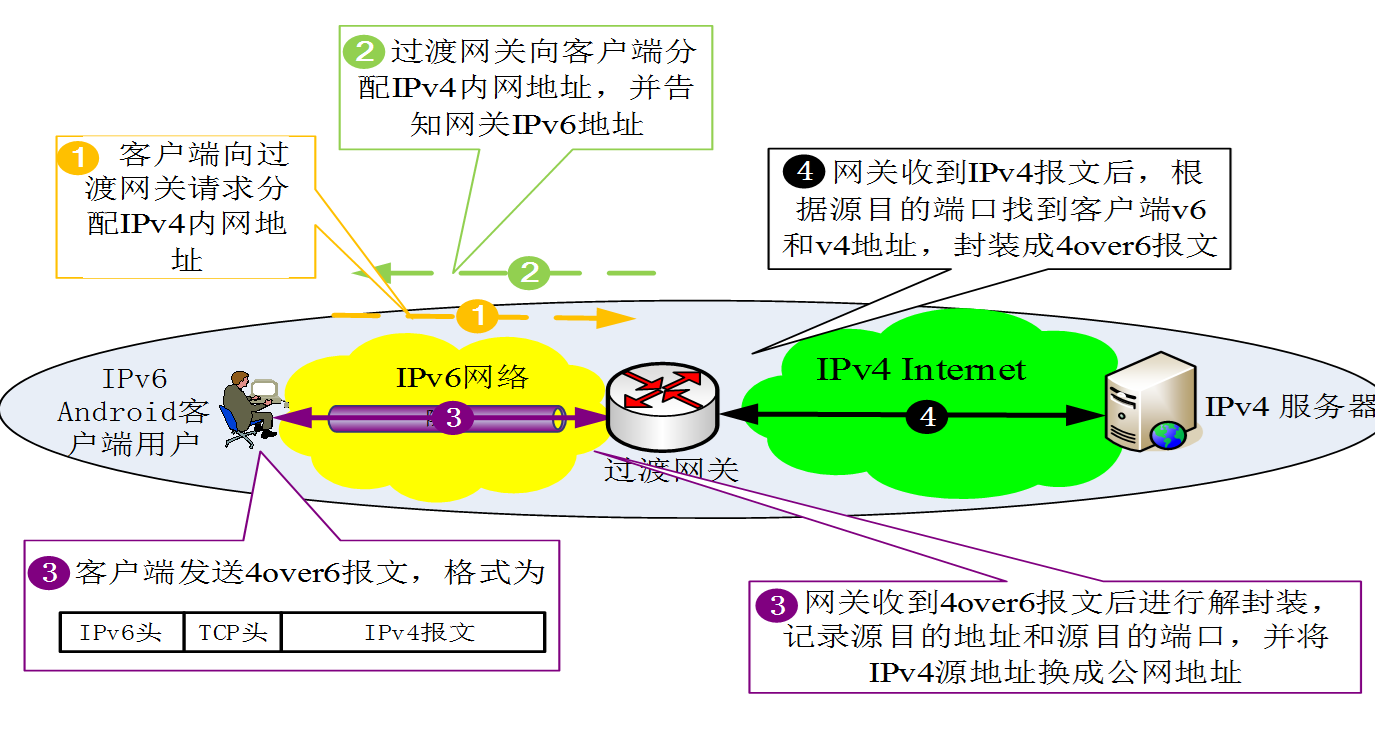
\includegraphics[width=\textwidth]{fig1}
\caption{4over6隧道模式原理图}
\end{figure}

IPv4 over IPv6隧道模式是指,将IPv4的报文装载到IPv6网络的数据段,通过隧道模式进行传递,这样就可以使用IPv6的网络来访问IPv4的资源。主要流程如下:

安卓客户端向过渡网关请求分配IPv4内网地址;过渡网关分配IPv4内网地址,并提供对应的IPv6网络地址;接着,安卓客户端发送4over6报文,过渡网关接受报文并进行分析,得到源地址和目的地址,将IPv4地址转化为公网地址,发送到公网之中;当过渡网关收到公网的IPv4报文之后,根据记录好的映射关系,重新封装成4over6报文,发给对应的内网用户,完成数据的转发和接受。

在以上流程中,用户处于IPv6的网络环境之中,过渡网关横跨IPv4和IPv6,并在其中提供IPv4和IPv6地址的转换和分发。在本实验中,过渡网关部分的代码已经完成,我们需要完成用户端的代码,以实现IPv4 over IPv6隧道协议。

\subsection{安卓VPN Service原理}

在本实验中,我们采用了VPN Service作为基本框架来实现IPv4 over IPv6隧道协议。VPN Service是安卓提供的一套API接口,方便编程人员创建VPN服务。当打开该服务之后,安卓系统将所有应用程序发送的IP包都根据iptables,使用NAT转发到TUN虚拟网络设备上,其端口为tun0。当打开VPN Service之后,我们可以获取tun0的文件描述符,这样就可以读取或者写入数据以实现发送或者接收数据。

也就是说,在打开VPN Service之后,我们可以监控系统所有的网络进程,并从tun中获得系统中所有IP包。这样,我们就可以将IP包封装在IPv6报文之中,使用隧道协议将报文发送到服务器,实现数据的发送;当我们收到服务器反馈的IPv6报文后,我们将其进行拆解,得到真正的IPv4包,再写入到tun文件之中,以实现数据的接收。

\subsection{JNI与NDK}

在本次实验中,由于经常要和以字节为单位的数据打交道,并且需要精细地管理内存,因此我们采用C来实现IPv4 over IPv6的核心功能。要在以Java为语言的安卓环境中使用C来进行编程,我们需要使用JNI和NDK。

Java Native Interface(JNI)规定了一套Java的原生接口,规定了Java和其他语言交互或者是在其他平台下运行时的接口,让我们可以使用其他语言(如C、C++、汇编等)访问Java中的类和对象。而Native Development Kit(NDK)是Google提供的一套方便开发者的开发套装(SDK),方便编程人员将C或者C++程序打包并加入到APK之中,供安卓程序使用。

\section{实验设计与内容}

\subsection{程序整体设计流程}

本次实验的编码主要分为两个部分,Java实现的安卓客户端(前端)和C实现的收发进程(后端),前端和后端之间通过管道(named pipe)来进行连接并传递数据。实验整体流程如下:

// TODO

\subsection{前端工作流程}



\subsection{后端工作流程}



\subsection{前端与后端的交互和通讯}



\section{实验结果与分析}



\section{实验中遇到的问题}



\section{实验心得与体会}



\section{对实验的意见和建议}


\end{document}
